\begin{center}{ \bf  РАСЧЕТ НЕРАВНОМЕРНОСТИ РАСПРЕДЕЛЕНИЯ КОМПОНЕНТА ПО ОХЛАЖДАЮЩИМ КАНАЛАМ КАМЕРЫ ЖИДКОСТНОГО РАКЕТНОГО ДВИГАТЕЛЯ НА ОСНОВЕ МОДЕЛИРОВАНИЯ В ANSYS CFX}\\
{\it Д.Н. Галдин, Т.И. Дарнева, А.В. Кретинин, А.Н. Попков} \\
(г.Воронеж, ВГТУ)
\end{center}
\addcontentsline{toc}{section}{Галдин Д.Н., Дарнева Т.И., Кретинин А.В., Попков А.Н.\dotfill}

Проточная часть регенеративной системы охлаждения камеры жидкостного ракетного двигателя
образована множеством однотипных каналов с коллекторным подводом и отводом охлаждающего компонента топлива.
Данное конструктивное оформление исследуемой системы заранее пре\-д\-полагает
наличие неравномерности распределения давления и расхода по длине коллекторов и по отдельным каналам тракта охлаждения.
Величина данной неравномерности может составлять величину более 10 $\%$
и это приводит к снижению надёжности наружного охлаждения стенки камеры.
На величине неравномерности распределения охладителя могут сказаться
и особенности технологии изготовления паяной двуслойной конструкции рубашки охлаждения,
что неизбежно сказывается на различных коэффициентах гидравлического сопротивления отдельных каналов,
не говоря уже о возможности возникновения <<запаев>> каналов, что приводит к резкому снижению расхода через такие каналы.

Всестороннее влияние всей совокупности факторов на величины расходов охладителя в отдельных каналов
в настоящее время не может быть исследовано с достаточной надёжностью.
Поэтому, принимая <<неизбежность>> данной проблемы, т.е. то, что она присутствует практически во всех ЖРД,
и соглашаясь т.о. на стохастическую природу исследуемой проблемы, важно выявить эпистемические неопределённости,
формирующие значительную часть величины неравномерности,
которые мы можем выявить и убрать их из общей совокупности неопределённостей
и т.о. снизить величину негативной расходной неравномерности.
С этой целью осуществлялось численное моделирование гидродинамики регенеративной системы охлаждения с использованием инструментария ANSYS Workbench.

На рисунке 1 приведена исследуемая геометрическая модель проточной части охлаждающего тракта камеры сгорания,
состоящая из 101 канала в совокупности с коллекторами подвода и сбора охладителя,
построенная в модуле ANSYS Design Modeler.

При построении расчётного блока осуществляется синтез математический модели исходя из возможностей модуля ANSYS CFX, т.е. выбирается модель турбулентности, подключается уравнение энергии для моделирования гидродинамики с теплообменом, осуществляется соответствующая постановка граничных условий, устанавливаются параметры сходимости: максимальное количество итераций и RMS ошибка в критерии сходимости. Основными результатами расчёта являются значения расходов через отдельные каналы тракта охлаждения.

На рисунке 2 приведены линии тока движущейся жидкости в проточной части исследуемой системы регенеративного охлаждения цилиндрической камеры сгорания.

На рисунке 3 представлены некоторые результаты расчёта распределения компонента по каналам охлаждающего тракта,
проведённого при изменении ряда граничных условий.
Вариант <<Противоток>> означает,
что подводящие штуцеры подвода и отвода компонента расположены диаметрально с противоположных сторон камеры.
Вариант <<Выход+1>> также рассчитан для случая противотока,
но со смещением выходного штуцера на один градус от перпендикулярного исполнения.
Вариант <<Смещение входа 2 гр>> рассчитан для случая противотока со смещением входного штуцера на 2 градуса от перпендикулярного исполнения.

\begin{figure}
	\centering
	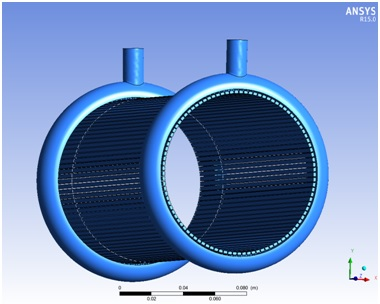
\includegraphics[width=0.9\textwidth]{GALDIN1.jpg}
	\caption{Геометрическая модель проточной части охлаждающего тракта камеры сгорания}
\end{figure}

\begin{figure}
	\centering
	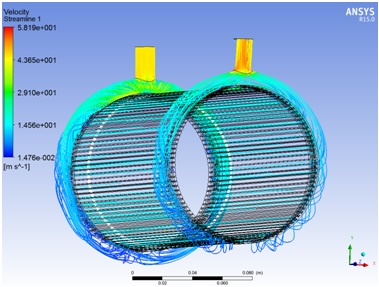
\includegraphics[width=0.9\textwidth]{GALDIN2.jpg}
	\caption{Линии тока в проточной части охлаждающего тракта камеры сгорания}
\end{figure}

Вариант <<Прямоток>> означает, что подводящие штуцеры подвода и отвода компонента расположены с одной стороны камеры. Вариант <<Вход 2гр с одной стороны>> рассчитан для случая прямотока со смещением входного штуцера на 2 градуса от перпендикулярного расположения. И, наконец, вариант <<С теплообменом>> рассчитан для сопряжённой задачи моделирования гидродинамики с наличием подвода тепла в охладитель.
\begin{figure}
	\centering
	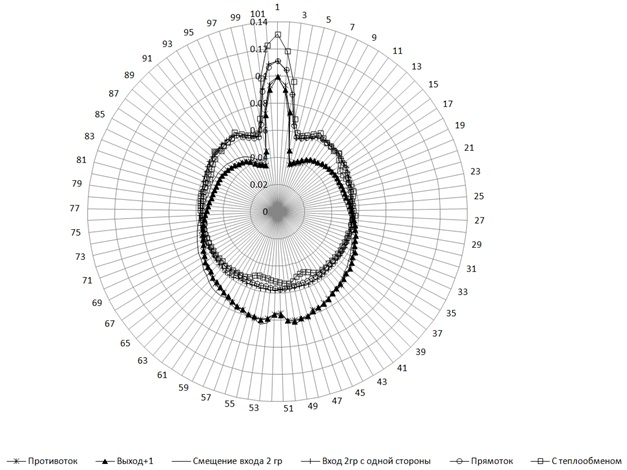
\includegraphics[width=0.9\textwidth]{GALDIN3.jpg}
	\caption{Результаты распределения охладителя по отдельным каналам охлаждающего тракта камеры сгорания при различных вариантах конструктивного исполнения}
\end{figure}

Анализируя проведённые расчёты, можно отметить следующие результаты:
\begin{itemize}
	\item
	в охлаждающих каналах напротив подводящего штуцера наблюдаются повышенные расходы, причём величина расхода в канале номер 1 может превышать средние значения расходов более чем в 2 раза. Влияние подводящего штуцера сказывается на порядка 10 $\%$ всех каналов системы, обуславливая пониженные значения расходов через остальные 90 $\%$ каналов;

	\item
	для охлаждения <<хуже>> пониженные значения расходов через каналы. Поэтому, судя по рисункам, схема <<прямоток>> предпочтительнее схемы <<противоток>>;

	\item
	неперпендикулярное исполнение штуцеров подвода и отвода охладителя приводят к изменению расходов через каналы максимум на 4-5 $\%$;

	\item
	наличие теплового потока в охладитель ещё более увеличивает величину расходной неравномерности.
\end{itemize}
\smallskip \centerline{\bf Литература}\nopagebreak

1. {\it Кретинин А.В., Булыгин Ю.А., Климов В.Ю., Дронов П.А.} Стохастический расчёт распределения расхода по каналам тракта охлаждения камеры жидкостного ракетного двигателя. Известия высших учебных заведений. Авиационная техника. 2009. № 4. C. 42-44.

2. {\it Кретинин А.В., Булыгин Ю.А., Ткаченко Ю.С.} Недетерминированное моделирование теплофизических процессов в камере жидкостного ракетного двигателя. Вестник Воронеж. гос. техн. ун-та. 2013. Т. 9. № 1. С. 88-92.
